\section{Presentation of the Web-based Platform}

%     interface
%     hosting final product in docker containers and charge balancing with nginx


\subsection{Introduction}
    In this section we are going talk about the different tools and resources that helped us build our project, we will talk about the software, hardware and explain in detail the features of the web application and finally present the interface.


\subsection{Hardware}
    This project is a 2 person teamwork, we were able to impliment it using 2 laptops: \\
    \bigskip \\
    \textbf{Asus vivobook}: with an intel CPU i7 7nth generation with a clock rate of 2.7GHz and an Nvidia GPU Geforce 930mx, 12 GB of RAM and 240GB of Solid State Drive, with a Linux Mint 20.3 Cinnamon operating system\\ 
    \bigskip \\
    \textbf{Dell XPS}: with a 7th Generation Intel Core i7-7700HQ Quad Core Processor (6M cache, up to 3.8 GHz) and NVIDIA GeForce GTX 1050 4GB DDR5 Graphics that was used to train the CNN model , 16 GB RAM DDR4-2400MHz and 512GB PCIe Solid State Drive, with a Windows 10 professional edition operating system \\ 


\subsection{Software}
    The implemetation of the project was acheived using various frameworks and libraries, and from those we mention the following: \\
    \begin{itemize}
        \item 1
        \item 2
        \item 3
        \item 4
    \end{itemize}

\subsection{The Web Application}
    \subsubsection{Authentication}
        The Authentication was implimented using JWTs (json web tokens) which is aquired by the frontend client after Loging in or Signing up, after that it will be saved in a session storage and sent as an Authorization header with each request that requires authentication, in the backend the tokens are saved in an array to allow for multiple session communication, which means that a user can connect from multiple devices, with the ability to logout from all sessions being available in the profile settings.
    
    \subsubsection{Permissions and Roles}
        There are mainly 3 roles in our application: Admin, Doctor, User. Each one of these roles commes with a certain level of access. The permissions were implimented using ExpressJS middleware, the list of permissions goes as follows, 

        \begin{description}
            \item[Admin]:\\
            \begin{itemize}
                \item User manegment.
                \item View all doctors
                \item Docotr verification, through credentials sent by e-mail.
            \end{itemize}
            \item[Docotr]:\\
            \begin{itemize}
                \item View published lesions.
                \item Comment on a published lesion
                \item Communicate with a patient
            \end{itemize}
            \item[User]:\\
            \begin{itemize}
                \item Profile managment.
                \item Upload a lesion.
                \item Publish/Unpublish a lesion
                \item View own lesions
                \item Comment  on own lesion
                \item Communicate with a doctor 
            \end{itemize}
        \end{description}
    
        Keep in mind that the Admin also has the permissions of the doctor, and a Doctor also has the permissions of a normal user.

    \subsubsection{Communications Between Different Parts Of The Application}
        We devided our application 2 frontends and 2 backends and a database, 2 frontend clients one for a browser(ReactJS) and one for a smartphone (Flutter), these 2 communicate with the main backend (NodeJS) using Rest API architecture and http/https protocol. and the main backend communicates with the 2nd backend (flask) which has the implementation of the CNN prediction model also using Rest API architecture and http/https protocol, and with the databse server using MongoDB protocol.

        The CNN model is used when a user uploads a lesion image to the NodeJS backend, and after that the Node server sends the image to the model and receives a prediction string from it which after that saved in the database and returned to the fronend client.

    \subsubsection{Hosting}
    Docker...
    hosting diagram

    \subsubsection{The Interface}
        We present the application's interface in the following figures: 
        % ---login 
        % ---signup
        % profile
        %     lesions
        %         ---upload 
        %         ---previous lesions
        %     settings
        %         ---upload photo
        %         delete photo
        %         ---delete account
        %         logout all
        % ---forum
        % ---messages
        % dashboard
        %     ---doctors, verify unverify
        %     users, delete



        % \begin{figure}[H]
        % \begin{center}
        % \includegraphics[width=12cm]{./diagnosis-system/presentation-of-app/.png}
        % \end{center}
        % \caption{}
        % \label{fig:}
        % \end{figure}

        
        \noindent \textbf{First of all, the following 2 figures demonstrate the Login and Signup interfaces:} \\
        you can login with Email and Password, or Signup providing Name, Role, Email, Password
        \begin{figure}[H]
        \begin{center}
        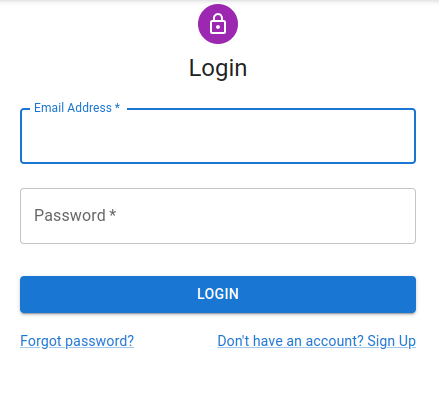
\includegraphics[width=7cm]{./diagnosis-system/presentation-of-app/login.png}
        \end{center}
        \caption{Login}
        \label{fig:}
        \end{figure}

        

        \begin{figure}[H]
        \begin{center}
        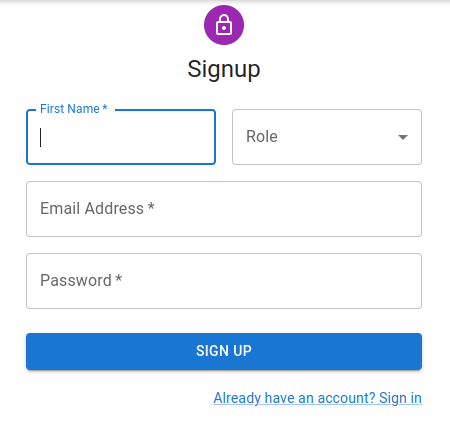
\includegraphics[width=7cm]{./diagnosis-system/presentation-of-app/signup.png}
        \end{center}
        \caption{Signup}
        \label{fig:}
        \end{figure}

        
        \noindent \textbf{The following interfaces are in the Profile page:} \\
        \noindent You can view profile information, upload a profile image, and delete your account 
        \begin{figure}[H]
        \begin{center}
        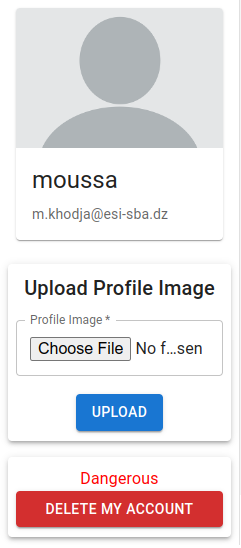
\includegraphics[width=7cm]{./diagnosis-system/presentation-of-app/profile-settings.png}
        \end{center}
        \caption{Profile Settings}
        \label{fig:}
        \end{figure}

        
        \noindent This component allows you to upload a lesion image with a description 
        \begin{figure}[H]
        \begin{center}
        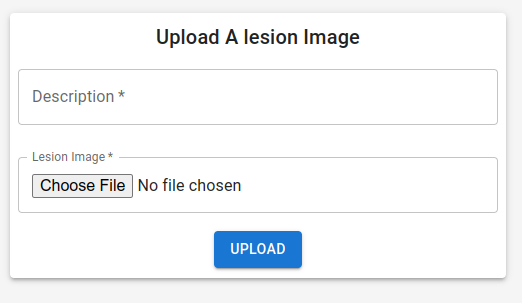
\includegraphics[width=10cm]{./diagnosis-system/presentation-of-app/upload-lesion.png}
        \end{center}
        \caption{Upload a lesion Image, with a description}
        \label{fig:}
        \end{figure}

        
        \noindent \textbf{The following interfaces are found in the Forum page:} \\
        \noindent You can view all lesions that were published by patients, and give your professional opinion by leaving a comment, you can also view comments from other doctors
        \begin{figure}[H]
        \begin{center}
        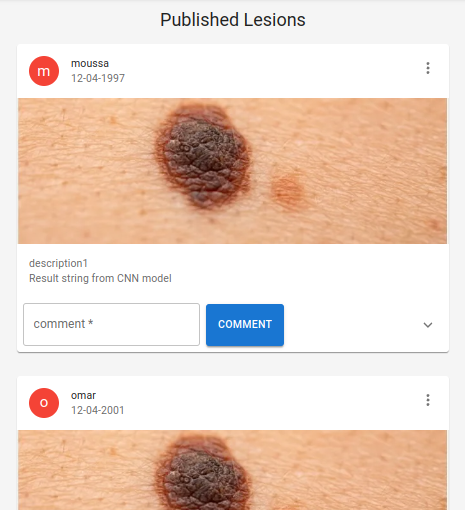
\includegraphics[width=10cm]{./diagnosis-system/presentation-of-app/published-lesions.png}
        \end{center}
        \caption{View published lesions as a doctor}
        \label{fig:}
        \end{figure}

        

        \begin{figure}[H]
        \begin{center}
        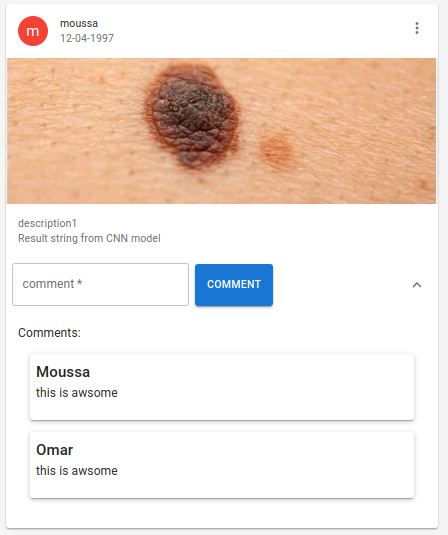
\includegraphics[width=10cm]{./diagnosis-system/presentation-of-app/comment.png}
        \end{center}
        \caption{Comment on a lesion}
        \label{fig:}
        \end{figure}

        
        \noindent \textbf{This interface represents the Communication page:} \\
        You can send and reveive messages, between doctors and patients
        \begin{figure}[H]
        \begin{center}
        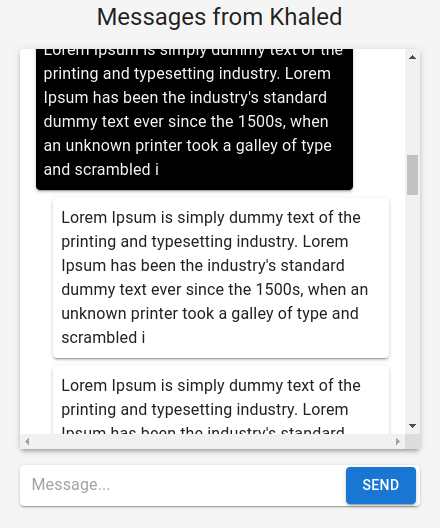
\includegraphics[width=10cm]{./diagnosis-system/presentation-of-app/messeges.png}
        \end{center}
        \caption{Messaging}
        \label{fig:}
        \end{figure}

        
        \noindent \textbf{The folowing interfaces are found in the dashboard:} \\
        After checking the credentials sent by email, the admin can verify a doctor's account, because a non-verified doctor is considerd as a normal user and he cant access patients information 
        \begin{figure}[H]
        \begin{center}
        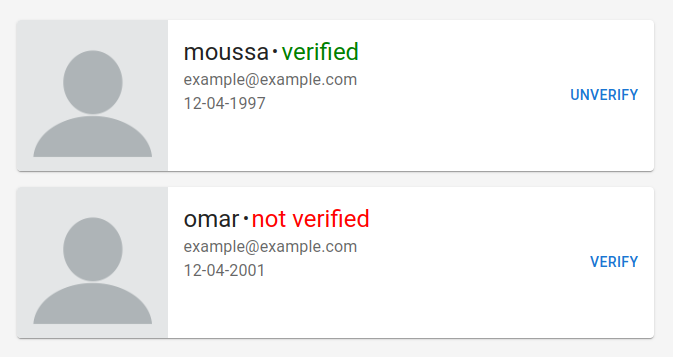
\includegraphics[width=10cm]{./diagnosis-system/presentation-of-app/verify-doctors.png}
        \end{center}
        \caption{View all doctors by Admin + verify/Unverify a doctor}
        \label{fig:}
        \end{figure}


        
        
\subsection{Future Work}
    we present these ideas as a future work to extend the usability of our project
    \begin{itemize}
        \item Detect and classify more lesions and not just melanoma.
        \item Take model interpritability into account, so it will be more acceptable in real world scenarios.
        \item Present more in-app features to facilitate and enhance user experience. 
    \end{itemize}